(1): $\ve{b} = \ve{\rm AB}$, $\ve{c} = \ve{\rm AC}$, $\ve{d} = \ve{\rm AD}$とおく. このとき$\ve{\rm AP}, \ve{\rm AQ}, \ve{\rm AR}$は実数$0\leq p,q,r\leq 1$を用いて
\bealn{
\ve{\rm AP} &= p(\ve{b} + \ve{d}) \\
\ve{\rm AQ} &= q(\ve{c} + \ve{d}) + (1-q)\ve{b} \\
\ve{\rm AR} &= r\ve{d} + (1-r)\ve{c}
 }
 と表せるので, $\ve{\rm AG} = \dfrac{1}{3}\parena{\ve{\rm AP} + \ve{\rm AQ} + \ve{\rm AR}}$を計算すると
 \[
 \ve{\rm AG} = \dfrac{1}{3}(1 + p-q)\ve{b} + \dfrac{1}{3} (1 + q-r)\ve{c} + \dfrac{1}{3} (p+q+r)\ve{d}
 \]
 となる. ここで$|\ve{d}| = 1$より, $\dfrac{1}{3}(p+q+r)$はちょうど${\rm G}$の面${\rm ABC}$から見た高さに一致することに注意する. $S(t)$を考察するために, $\dfrac{1}{3}(p+q+r) = t$とおいて固定する($0\leq t\leq 1$). ${\rm AP} = t$なる点${\rm P}$を線分${\rm AD}$上にとると, $\ve{\rm AP} = t\ve{d}$なので${\rm P}$と$K$の高さ$t$の部分は同一平面上にあり,
 \bealn{
 \ve{\rm AG} - \ve{\rm AP} = \ve{\rm PG} =  \dfrac{1}{3}(1 + p-q)\ve{b} + \dfrac{1}{3} (1 + q-r)\ve{c}.
 }
 となる.  $r = 3t - p - q$ を代入すると
 \bealn{
 \ve{\rm PG} &=  \dfrac{1}{3}(1 + p-q)\ve{b} + \dfrac{1}{3} (1 + q + 2q - 3t)\ve{c}\\
 &= \parena{\dfrac{1}{3}\ve{b} + \dfrac{1-3t}{3}\ve{c}} + \dfrac{p-q}{3}\ve{b} + \dfrac{p+2q}{3}\ve{c} \\
 &= \parena{\dfrac{1}{3}\ve{b} + \dfrac{1-3t}{3}\ve{c}} \\
 &\qquad\qquad + p\parena{\dfrac{1}{3} \ve{b} + \dfrac{1}{3} \ve{c}} + q\parena{\dfrac{2}{3}\ve{c} - \dfrac{1}{3}\ve{b}} \\
 }
 である. ここで, 第一項は$t$にのみ依存するベクトルである. よって$t$が固定されているもとでは, ${\rm G}$が通過する領域は
 \[
 p\ve{x} + q\ve{y} \quad \text{ただし} \ve{x} =\dfrac{1}{3} \ve{b} + \dfrac{1}{3} \ve{c},\quad \ve{y} = \dfrac{2}{3}\ve{c} - \dfrac{1}{3}\ve{b}
 \]
 というベクトルの終点が, $0\leq p\leq 1$, $0\leq q\leq 1$, $0\leq r = 3t-p-q \leq 1$のもとで動かしたときに通過する領域を平行移動したものであり, その面積もまた$S(t)$である. \par
 ここで$0\leq t\leq \frac{1}{3}$とおく. $0\leq 3t-p-q\leq 1$を変形すると$3t-1\leq p+q\leq 3t$である. $t$を$t+\frac{1}{3}$に置き換えると$3t \leq  p + q \leq 3t + 1$となり, $t + \frac{2}{3}$に置き換えると$3t + 1 \leq p+q \leq 3t + 2$となる.

 よって面積の和$S(t) + S(t+\frac{1}{3}) + S(t+\frac{2}{3})$は, $p\ve{x} + q\ve{y}$の終点が,
 \[0\leq p\leq 1,\quad 0\leq q\leq 1,\quad 3t-1 \leq p + q \leq 3t + 2\]
 のもとで動かしたときに通過する領域の面積に一致する. また, 3番目の条件は$3t - 1 \leq 0$, $2\leq 3t+2$によって実際は不要である. したがって$0\leq p,q\leq 1$のもとで動かしたときの$p\ve{x} + q\ve{y}$の終点が通過する領域の面積となるので, $t$によらず一定である. \\
 (2): (1)による一定値を$T$とおく. $K$の体積は$S(t)$の積分として求められるが,
 \bealn{
 &\int_{0}^{1}S(t) \, dt \\
 &= \int_{0}^{\frac{1}{3}} \parena{S(t) + S\parena{t+ \frac{1}{3}} + S\parena{t + \frac{2}{3}}}\, dt \\
 &= \int_{0}^{\frac{1}{3}} T \, dt = \dfrac{T}{3}
 }
 のように$k$で表せるので, $T$を求めよう. \par
 $T$は$p\ve{x} + q\ve{y}$ ($0\leq p,q\leq 1$)の終点の通貨する領域の面積であり, これは$\ve{x}, \ve{y}$で張られる平行四辺形の面積に一致する. よって, $\ve{x}, \ve{y}$のなす角を$\theta$とすれば
 \bealn{
 T&=2\times \dfrac{1}{2}|\ve{x}||\ve{y}|\sin{\theta}
 }
 となる. 下図において${\rm M}$は${\rm BC}$の中点, ${\rm N}$は${\rm BC}$を$2:1$に外分する点とすると,
 $\frac{3}{2} \ve{x} = \ve{\rm AM}$, $3\ve{y} = \ve{\rm AN}$である. とくに$\ve{x}, \ve{y}$のなす角$\theta = \angle{\rm NAM}$は, $\triangle{\rm NAM}$が直角三角形でかつ${\rm NM}: {\rm AM} = 3{\rm CM}:\sqrt{3}{\rm CM} = \sqrt{3}:1$ であることから$\theta = 60^{\circ}$である. また, ${\rm AM} = \dfrac{\sqrt{3}}{2}$, ${\rm AN} = \dfrac{{\rm AM}}{\cos{\theta}} = \sqrt{3}$も得られるので
 \[|\ve{x}| = \dfrac{2}{3}{\rm AM} = \dfrac{\sqrt{3}}{3}, \quad |\ve{y}| = \dfrac{1}{3}{\rm AN} = \dfrac{\sqrt{3}}{3}\]
 となる. 以上より, $K$の体積は
 \[
 \dfrac{T}{3} = \dfrac{|\ve{x}||\ve{y}|}{3}\sin{60^{\circ}} = \bolm{\dfrac{\sqrt{3}}{18}}
 \]
\begin{center}
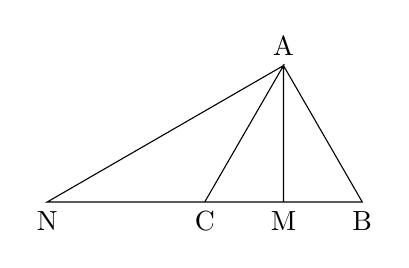
\begin{tikzpicture}
\draw (0,0)node[below]{M}--(-3,0)node[below]{N}--(0,1.732)node[above]{A}--(-1,0)node[below]{C}--(1,0)node[below]{B}--(0,1.732)--(0,0);
\end{tikzpicture}
\end{center}
 % となる. 内積と絶対値を計算すると, $\ve{b}\cdot \ve{c} = \frac{1}{2}$, $|\ve{b}| = |\ve{c}|=1$により
 % \bealn{
 % |\ve{x}|^2 &= \dfrac{|\ve{b}|^2}{9} + \dfrac{2(\ve{b}\cdot \ve{c})}{9} + \dfrac{|\ve{c}|^2}{9} = \dfrac{1}{3} \\
 % |\ve{y}|^2 &= \dfrac{|\ve{b}|^2}{9} - \dfrac{4(\ve{b}\cdot \ve{c})}{9} + \dfrac{4|\ve{c}|^2}{9} = \dfrac{1}{3} \\
 % \ve{x}\cdot \ve{y}
 %}
